\documentclass{article}
\usepackage[margin=1in]{geometry}
\usepackage[utf8]{inputenc}
\usepackage{hyperref}
\usepackage{algorithm2e}

\renewcommand\UrlFont{\color{blue}\rmfamily}

%%%%% MATH %%%%%
\usepackage{amsmath,amsthm,amsfonts,amssymb,mathtools}
%\usepackage[libertine]{newtxmath}
\usepackage[bold,small,basic]{complexity}

%%%%% TIKZ AND PICS %%%%%
\usepackage{graphicx}
\usepackage[framemethod=TikZ]{mdframed}
\usepackage{tikz, float, caption, subcaption}
\captionsetup{compatibility=false}
\usetikzlibrary{arrows, automata, positioning, fit, shapes.geometric}

%%%%% FORMATTING %%%%%
\usepackage{enumitem, fancyhdr, multicol}
\usepackage{booktabs}
\usepackage[numbers]{natbib}

%%%%% 0-Ary Macros %%%%%

%% Strings %%
\newcommand{\emptystr}{\varepsilon}
\newcommand{\blank}{\text{\textvisiblespace}}
\newcommand{\0}{\mathbf{0}}
\newcommand{\1}{\mathbf{1}}
\newcommand{\2}{\mathbf{2}}

%% Sets and Langs %%
\newcommand{\nats}{\mathbb{N}}
\newcommand{\ints}{\mathbb{Z}}
\newcommand{\rats}{\mathbb{Q}}
\newcommand{\reals}{\mathbb{R}}
\newcommand{\complexes}{\mathbb{C}}
\newcommand{\TQBF}{\lang{TQBF}}
\newcommand{\RCG}{\lang{RCG}}
\newcommand{\CNFSAT}{\lang{CNFSAT}}

%% Logic Symbols %%
\newcommand{\myand}{\mathrel{\wedge}}
\newcommand{\myor}{\mathrel{\vee}}
\newcommand{\mynot}{\neg}
\newcommand{\st}{\mid}
\newcommand{\turnstile}{\vdash}
\newcommand{\turnstar}{\overset{*}{\vdash}}
\newcommand{\False}{\textsc{False}}
\newcommand{\True}{\textsc{True}}
\renewcommand{\p}{\varphi}

%%%%% Larger-Ary Macros %%%%%

%% Sets, Containers, and Functions on Them %%
\newcommand{\set}[1]{{\left\{{#1}\right\}}}
\newcommand{\card}[1]{{\|{#1}\|}}
\newcommand{\powset}[1]{\mathcal{P} \left({#1}\right)}
\newcommand{\tup}[1]{\langle{} #1 \rangle{}}

\newcommand{\Turnstile}[1]{\underset{#1}{\turnstile}}
\newcommand{\Turnstar}[1]{\underset{#1}{\overset{*}{\vdash}}}

%% Fonts %%
\newcommand{\tb}[1]{\textbf{#1}}
\newcommand{\bs}[1]{\boldsymbol{#1}}
\newcommand{\mbf}[1]{\mathbf{#1}}

%% Functions %%
\newcommand{\reduc}[3]{{{#1} \le_{#3} {#2}}}
\newcommand{\reducp}[2]{{{#1} \le_p {#2}}}
\newcommand{\reducm}[2]{{{#1} \le_m {#2}}}
\newcommand{\map}[3]{{{#1}:{#2}\rightarrow{#3}}}

%%%%% FIGURE FORMATTING %%%%%
\captionsetup[figure]{labelfont={bf, it},textfont={it}}
\captionsetup[subfigure]{labelfont=bf,textfont=normalfont}

%%%%% VARS %%%%%
\newcounter{row}
\newcounter{col}

\newcommand\drawgrid[2]{
  \begin{tikzpicture}[scale=0.7]
    \edef\rowMatrix{#2}
    %% Find the extents
    \edef\nRow{0}

    \foreach \row in \rowMatrix {
      \edef\nCol{0}
      \foreach \col in \row {
        \pgfmathparse{\nCol + 1}
        \xdef\nCol{\pgfmathresult}
      }
      \pgfmathparse{\nRow + 1}
      \xdef\nRow{\pgfmathresult}
    }

    \pgfmathparse{\nRow - 1}
    \edef\nRow{\pgfmathresult}

    \foreach [count=\rowIx] \row in \rowMatrix{
      \foreach [count=\colIx] \elem in \row{
        \def\x{\colIx - 1}
        \pgfmathdivide{\rowIx - 1}{3}
        \def\y{1 - \rowIx}
        \node at (\x + 0.5, \y - 0.5) {$\elem$};
      }
    }
    \draw[thick] (1,  0) -- (1, -\nRow);
    \draw[thick] (#1,  0) -- (#1, -\nRow);

    \draw[thick] (0, -1) -- (\nCol, -1);
    \draw[thick] (0, -2) -- (\nCol, -2);
  \end{tikzpicture}
}

\newcommand\drawgame[1]{
  \begin{tikzpicture}[scale=0.7]
    \edef\rowMatrix{#1}
    %% Find the extents
    \edef\nRow{0}

    \foreach \row in \rowMatrix {
      \edef\nCol{0}
      \foreach \col in \row {
        \pgfmathparse{\nCol + 1}
        \xdef\nCol{\pgfmathresult}
      }
      \pgfmathparse{\nRow + 1}
      \xdef\nRow{\pgfmathresult}
    }

    \pgfmathparse{\nRow - 1}
    \edef\nRow{\pgfmathresult}

    \draw[thick] (0, 0) grid (\nCol, - \nRow);
    \draw[very thick, white] (\nCol, 0) -- (\nCol, -\nRow);
    \draw[very thick, white] (0, -\nRow) -- (\nCol, -\nRow);

    \foreach [count=\rowIx] \row in \rowMatrix{
      \foreach [count=\colIx] \elem in \row{
        \def\x{\colIx - 1}
        \pgfmathdivide{\rowIx - 1}{3}
        \def\y{1 - \rowIx}
        \node at (\x + 0.5, \y - 0.5) {${\elem}$};
      }
    }
  \end{tikzpicture}
}

\newcommand\DrawGame[3]{
  \begin{tikzpicture}[scale=0.7]
    \edef\rowMatrix{#3}
    %% Find the extents
    \edef\nRow{0}

    \foreach \row in \rowMatrix {
      \edef\nCol{0}
      \foreach \col in \row {
        \pgfmathparse{\nCol + 1}
        \xdef\nCol{\pgfmathresult}
      }
      \pgfmathparse{\nRow + 1}
      \xdef\nRow{\pgfmathresult}
    }

    \pgfmathparse{\nRow - 1}
    \edef\nRow{\pgfmathresult}

    \colorlet{fill}{gray!30}
    \fill[color=fill] #1 rectangle #2;

    \draw[thick] (0, 0) grid (\nCol, - \nRow);
    \draw[very thick, white] (\nCol, 0) -- (\nCol, -\nRow);
    \draw[very thick, white] (0, -\nRow) -- (\nCol, -\nRow);

    \foreach [count=\rowIx] \row in \rowMatrix{
      \foreach [count=\colIx] \elem in \row{
        \def\x{\colIx - 1}
        \pgfmathdivide{\rowIx - 1}{3}
        \def\y{1 - \rowIx}
        \node at (\x + 0.5, \y - 0.5) {${\elem}$};
      }
    }
  \end{tikzpicture}
}

\newcommand\DrawMidGame[3]{
  \begin{tikzpicture}[scale=0.7]
    \edef\rowMatrix{#3}
    %% Find the extents
    \edef\nRow{0}

    \foreach \row in \rowMatrix {
      \edef\nCol{0}
      \foreach \col in \row {
        \pgfmathparse{\nCol + 1}
        \xdef\nCol{\pgfmathresult}
      }
      \pgfmathparse{\nRow + 1}
      \xdef\nRow{\pgfmathresult}
    }

    \pgfmathparse{\nRow - 1}
    \edef\nRow{\pgfmathresult}

    \colorlet{fill}{gray!30}
    \fill[color=fill] #1 rectangle #2;

    \draw[thick] (0, 0) grid (\nCol, - \nRow);
    \draw[very thick, white] (0, 0) -- (\nCol, 0);
    \draw[very thick, white] (0, 0) -- (0, -\nRow);
    \draw[very thick, white] (\nCol, 0) -- (\nCol, -\nRow);
    \draw[very thick, white] (0, -\nRow) -- (\nCol, -\nRow);

    \foreach [count=\rowIx] \row in \rowMatrix{
      \foreach [count=\colIx] \elem in \row{
        \def\x{\colIx - 1}
        \pgfmathdivide{\rowIx - 1}{3}
        \def\y{1 - \rowIx}
        \node at (\x + 0.5, \y - 0.5) {${\elem}$};
      }
    }
  \end{tikzpicture}
}

\newcommand\DrawLeftGame[3]{
  \begin{tikzpicture}[scale=0.7]
    \edef\rowMatrix{#3}
    %% Find the extents
    \edef\nRow{0}

    \foreach \row in \rowMatrix {
      \edef\nCol{0}
      \foreach \col in \row {
        \pgfmathparse{\nCol + 1}
        \xdef\nCol{\pgfmathresult}
      }
      \pgfmathparse{\nRow + 1}
      \xdef\nRow{\pgfmathresult}
    }

    \pgfmathparse{\nRow - 1}
    \edef\nRow{\pgfmathresult}

    \colorlet{fill}{gray!30}
    \fill[color=fill] #1 rectangle #2;

    \draw[thick] (0, 0) grid (\nCol, - \nRow);
    \draw[very thick, white] (0, 0) -- (\nCol, 0);
    \draw[very thick, white] (\nCol, 0) -- (\nCol, -\nRow);
    \draw[very thick, white] (0, -\nRow) -- (\nCol, -\nRow);

    \foreach [count=\rowIx] \row in \rowMatrix{
      \foreach [count=\colIx] \elem in \row{
        \def\x{\colIx - 1}
        \pgfmathdivide{\rowIx - 1}{3}
        \def\y{1 - \rowIx}
        \node at (\x + 0.5, \y - 0.5) {${\elem}$};
      }
    }
  \end{tikzpicture}
}

\theoremstyle{plain}
\newtheorem{theorem}{Theorem}
\newtheorem{conj}[theorem]{Conjecture}
\newtheorem{question}[theorem]{Question}
\newtheorem{note}[theorem]{Note}

\newtheorem{lemma}[theorem]{Lemma}
\newtheorem{ulemma}[theorem]{Maybe a Lemma?}
\newtheorem{cor}[theorem]{Corollary}

\theoremstyle{definition}
\newtheorem{definition}[theorem]{Definition}
\newtheorem{assm}[theorem]{Assumption}

%%%%% NAME %%%%%
\begin{document}
\title{Complexity of Regex Crosswords}
\author{%
  Stephen Fenner \and Daniel Pad\'e%
}
\date{February 2019}
%\authorrunning{S. Fenner \and D. Pad\'e}
%\institute{University of South Carolina, Columbia SC 29201 USA}

%%%%% Document %%%%%
\maketitle
\begin{abstract}
  In a regular expression crossword puzzle, one is given two non-empty lists $\tup{\tup{R_1,\ldots, R_m}$ and $\tup{C_1, \ldots, C_n}}$ over some alphabet, and the challenge is to fill in an $m\times n$ grid of characters such that the string formed by the $i^\text{th}$ row is in $L(R_i)$ and the string in the $j^\text{th}$ column is in $L(C_j)$. We consider a restriction of this puzzle where all the $R_i$ are equal to one another and similarly the $C_j$.   We consider a 2-player version of this puzzle, showing it to be \lang{PSPACE}-complete.  Using a reduction from \lang{3SAT}, we also give a new, simple proof of the known result that the existence problem of a solution for the restricted (1-player) puzzle is \lang{NP}-complete. %\keywords{Complexity \and Regular expressions \and Regex crossword \and Picture language \and NP-complete}
\end{abstract}

\section{Introduction}

Regular expression crossword puzzles (regex crosswords, for short) share some traits in common with traditional crossword puzzles and with sudoku.  One is typically given two lists $R_1,\ldots,R_m$ and $C_1,\ldots,C_n$ of regular expressions labeling the rows and columns, respectively, of an $m\times n$ grid of blank squares.  The object is to fill in the squares with letters so that each row, read left to right as a string, \emph{matches} (i.e., is in the language denoted by) the corresponding regular expression, and similarly for each column, read top to bottom.  The solution itself may have some additional property, e.g., spelling out a phrase or sentence in row major order.

Regex crosswords have enjoyed some recent popularity, having been discussed in several popular media sources \cite{mikejuk:regex-crossword,Black:regex-crossword}, and thanks to some websites where people can solve the puzzles online \cite{rc,rcs}. Some variants of the basic puzzle have also been posed~\cite{MIT-Mystery-Hunt}.

A natural complexity theoretic question to ask is: How hard is it to solve a regex crossword in general?\footnote{Glen Takahashi posted this question to Stack Exchange in 2012~\cite{Takahashi:regex-crossword}, but it has been asked by others independently.}  The folklore answer---easy to show and apparently found by several people independently---is that it is \lang{NP}-hard, and the corresponding decision problem (``Does a solution exist?'') is \lang{NP}-complete.

In this paper, we consider two variations on the basic regex crossword puzzle: (1) a restriction of the puzzle where all the row regexes $R_1,\ldots,R_m$ are equal and all the column regexes $C_1,\ldots,C_n$ are equal; and (2) a 2-player game where players take turns attempting to fill in successive rows and columns of the grid.  Variation (2) can also be restricted to having equal row regexes and equal column regexes for the two players.  These variants have corresponding decision problems:  Let \lang{RC} be the solution existence problem for variation (1), \lang{RCG'} the first-player-win problem for variation (2), and \lang{RCG} the first-player-win problem for the restricted version of (2) (see Sections~\ref{sec:np} and \ref{sec:pspace} for precise definitions).  Our main result is that \lang{RCG'} and \lang{RCG} are both \lang{PSPACE}-complete (see Section~\ref{sec:pspace}, below).  We give explicit polynomial reductions from \lang{TQBF} to \lang{RCG'} and from \lang{RCG'} to \lang{RCG}.

The \lang{NP}-completeness of \lang{RC} was shown in~\cite{Fenner:regex-crossword},\footnote{In the same paper, a restriction of \lang{RC} where the unique row and column regexes are equal to \emph{each other} was also shown \lang{NP}-complete.} but the polynomial reduction used there was indirect and needlessly complicated for its purpose.  As a warm-up to our main result, we give a simple, straightforward polynomial reduction from \lang{3SAT} to \lang{RC}.

In the spirit of the Post Correspondence Problem in computability, our results have the pedagogical benefit of showing the hardness of some decision problems in automata theory that are simply stated and accessible to any undergraduate theory student.  The proofs given here are similarly accessible.

\subsection{Connections to other work}

Regex crossword techniques bear some similarity to results in cellular automata, to the Cook-Levin theorem, and to results of Berger from the 1960s showing the undecidability of tiling the plane with Wang tiles (the so-called ``domino problem''~\cite{Berger:domino-problem}, which was the first proof that there exist finite tile sets that tile the whole plane but only aperiodically).

The particular problems we study here are perhaps chiefly inspired by results in the theory of two-dimensional languages (picture languages) from formal language theory~\cite{GR:2d-languages}.  Given two regexes $R$ and $C$ for the rows and columns, respectively, the \emph{unbounded} $(R,C)$-crossword problem asks whether a solution grid exists of \emph{any size}.  One can show that the recognizable picture languages coincide exactly with the letter-to-letter projections of $(R,C)$-crossword solutions~\cite[Theorem~8.6]{GR:2d-languages} (except that the empty picture may also be included in the language).  Recognizable picture languages can be defined in terms of finite objects known as tiling systems~\cite{GR:rec-picture-languages} (cf.~\cite[Definition~7.2]{GR:2d-languages}), and given a tiling system $\mathcal{T}$, it is not hard to show that one can effectively find two regular expressions $R$ and $C$ (over some alphabet) and a projection $\pi$ that defines the same picture language as $\mathcal{T}$.  The existence problem for recognizable picture languages (``Given a tiling system, does it define a nonempty language?'') is known to be undecidable (\cite[Theorem~9.1]{GR:2d-languages}), and so, putting these results together, we get that the existence problem for unbounded $(R,C)$-crosswords is undecidable as well.  A much more direct reduction from the halting problem to unbounded $(R,C)$-crossword existence was given in~\cite{Fenner:regex-crossword}, where it was also shown that one could even fix the column regex $C$ once and for all, as well as restricting $R$ and $C$ to be over a binary alphabet.

The unbounded regex crossword problem naturally assumes one regex $R$ for all rows and one regex $C$ for all columns, since the number of rows and columns is unspecified.  This directly motivates us to impose similar restrictions on the bounded regex crossword problems we study here, where the dimensions of the grid are given as part of the input.

\bigskip

We give some basic concepts and definitions in Section~\ref{sec:prelims}.  Section~\ref{sec:np} gives our polynomial reduction from \lang{3SAT} to \lang{RC}.  This reduction suggests the technique we use to show our main results about 2-player crossword games in Section~\ref{sec:pspace}.  We give open problems in Section~\ref{sec:open}.

\section{Preliminaries}\label{sec:prelims}
We fix an alphabet $\Sigma$ once and for all and assume it contains the symbols $0$ and $1$ at least.  For the \lang{NP}-completeness result of Section~\ref{sec:np}, one can assume that $\Sigma = \{0,1\}$.  For the \lang{PSPACE}-completeness result of Section~\ref{sec:pspace}, it suffices that $\Sigma = \{0,1,2\}$.

\subsection{3SAT}\label{sec:3sat}
An instance of \lang{3SAT} is described by a Boolean formula $\p$ over $k$ variables $x_1,\ldots,x_k$, given in conjunctive normal form:
\begin{align*}
  \p \coloneqq C_i \land \cdots \land C_d
\end{align*}
where each $C_i$ is a clause of three literals (each a variable or its negation) connected by disjunctions:
\begin{align*}
  C_i \coloneqq \ell_{i,1} \lor \ell_{i,2} \lor \ell_{i,3}
\end{align*}

The question is, is $\p$ true (is it \emph{satisfied}) for some assignment of the variables. This is the canonical complete problem for \lang{NP}. In Section~\ref{sec:np} we show that the language \lang{RC} --- the language of $(R,C)$-crosswords --- is \lang{NP}-complete by giving reduction from \lang{3SAT}.

\subsection{TQBF}\label{sec:tqbf}

An instance of \TQBF{} is described by a closed Boolean formula $\p$, given in prenex normal form:
\begin{align}\label{eqn:qbf}
  \p \coloneqq \exists x_0 \forall y_0 \cdots \exists x_{k-1} \forall y_{k-1}\exists x_k
  \tilde{\p}(x_0, y_0, \ldots, x_{k-1}, y_{k-1}, x_k)
\end{align}
where $\tilde{\p}$ is a quantifier-free Boolean formula which can be assumed to be in conjunctive normal form with $c$ clauses and $2k+1$ variables, for some positive $c$ and $k$.

The sentence $\p$ is naturally viewed as a two-player game, where the players alternate choosing truth values for the variables in order, the first player wishing to make the formula $\tilde{\p}$ true and second player wishing to make it false.  The question to be answered is whether $\p$ is true when the quantified variables range over the Boolean values $\False$ and $\True$. \footnote{ More precisely, the question is whether the sentence $\exists x_0   \forall y_0 \cdots \exists x_{k-1} \forall y_{k-1}\exists x_k   [\tilde{\p}(x_0, y_0, \ldots, x_{k-1}, y_{k-1}, x_k) = \True]$ holds in the two-element Boolean algebra $(\{\False,\True\},\myand,\myor,\mynot)$. } That is, whether the first player has a winning strategy in the corresponding game.%%

As \lang{3SAT} is for \lang{NP}, \lang{TQBF} is the canonical complete problem for \lang{PSPACE}. In Section~\ref{sec:pspace}, \RCG{} --- the language of (R,C)-crossword games (defined below) with a winning strategy for the first player --- is \lang{PSPACE}-complete by reduction from \TQBF{}.

\section{(R,C)-crosswords}\label{sec:np}
For two given regexes $R$ and $C$ over $\Sigma$, an \emph{$(R,C)$-crossword solution} is a two-dimensional $m$ by $n$ grid of symbols from the alphabet. Interpreting rows and columns as strings, each row must match $R$ and each column must match $C$.

An \emph{$(R,C)$-crossword} is represented as a 4-tuple $\tup{0^m, 0^n, R, C}$ where the number of rows and columns are given in unary as $m$ and $n$, and $R$ and $C$ are row and column regexes over $\Sigma$ (defined in the usual way, using the operators $\cup$, $\|$, $*$, where $\|$ or juxtaposition both indicate concatenation).

\begin{definition}
  The language \lang{RC} is the set of all $(R,C)$-crosswords for which there exists an $(R,C)$-crossword solution of the given dimensions.
\end{definition}

\lang{RC} was shown to be \lang{NP}-complete
in~\cite{Fenner:regex-crossword} via an indirect, complicated reduction.  In this section, we give a much more straightforward polynomial reduction from \lang{3SAT} to \lang{RC}.

\subsection{The reduction}

Given a Boolean formula $\p$ with $k\ge 1$ variables and $d$ clauses as defined in Section~\ref{sec:3sat} above (where we can assume $d\ge 3$), we construct an instance $\tup{0^{d+1},0^{k+d},R,C}$ of \lang{RC} as follows: For $1 \le i \le d$, we define $t_i$ to be the regex
\begin{align*}
  t_i & = \0^{i-1}\1\0^{d-i} = \underbrace{\0 \cdots \0}_{i - 1} \1 \underbrace {\0 \cdots \0}_{d - i}\;. \\
  \shortintertext{Then we define}
  S   & = \1^d\0^*                                                                                        \\
  R   & = \left( \displaystyle \bigcup_{i=1}^{d} t_i R_i \right) \cup S                                   \\
  C   & = \1\left(\0^*\1\0^*\right) \cup \0(\0^* \cup \1^*)
\end{align*}
where $S$ is called the `spine,' and for $1\le i\le d$, \ $R_i$ is derived from the formula $\p$ as follows:
\begin{align*}
  R_i                                                  & = (a_{i,1} \cdots a_{i,k}) \cup (b_{i,1} \cdots b_{i,k}) \cup (c_{i,1} \cdots c_{i,k}) \\
  \shortintertext{where, for $1 \le j \le k$,} a_{i,j} & = \left\{
  \begin{array}{ll}
    \1           & \text{ if the first literal in the } i^{\text{th}} \text{ clause is } x_j            \\
    \0           & \text{ if the first literal in the } i^{\text{th}} \text{ clause is } \overline{x_j} \\
    (\1 \cup \0) & \text{ otherwise }
  \end{array}
  \right.
\end{align*}
and $b_{i,j},\;c_{i,j}$ are set similarly according to the second and third literals in each clause.

We show that $\p$ is satisfiable iff an $(R, C)$-crossword solution exists.

First, assuming that $\p$ is satisfiable, where $\tup{z_1, \ldots, z_k}$ is a satisfying assignment, then this sets up a $d+1$ by $d+k$ crossword solution of the following form:

\begin{figure}[H]
  \centering
  \drawgrid{5.9}{
    {      , c_1    , c_2    , c_3    , \ldots , c_{d}  , c_{d + 1} , \ldots , c_{d + k}},
    {r_0   , 1      , 1      , 1      , \ldots , 1      , 0         , \ldots , 0        },
    {r_1   , 1      , 0      , 0      , \ldots , 0      , z_1       , \ldots , z_k      },
    {r_2   , 0      , 1      , 0      , \ldots , 0      , z_1       , \ldots , z_k      },
    {\vdots, \vdots , \vdots , \ddots , \vdots , \vdots , z_1       , \ldots , z_k      },
    {r_c   , 0      , 0      , 0      , \ldots , 1      , z_1       , \ldots , z_k      },
  }
  \caption{Solution}\label{table:solution}
\end{figure}
Here, the first row is the spine (matching $S$); the block on the left below the spine is akin to an identity matrix; and the block on the right consists of columns where each column is either all $1$'s or all $0$'s (save the first element, which is always $0$), according to each $z_i$.  An overview representation is shown below:

\begin{figure}[H]
  \centering
  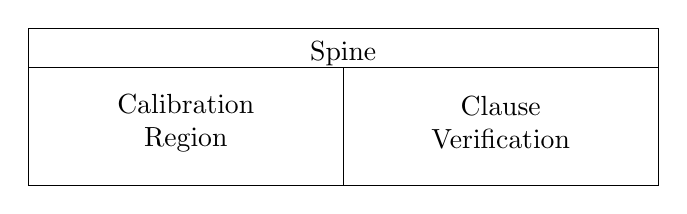
\begin{tikzpicture}
    \draw (0,0) rectangle (8,2);
    \draw (4,0) -- (4,1.5);
    \draw (0,1.5) -- (8,1.5);
    \node[anchor=south] at (4,1.4) {Spine};
    \node[align=center] at (2,0.8) {Calibration \\ Region};
    \node[align=center] at (6,0.8) {Clause \\ Verification};
  \end{tikzpicture}
\end{figure}

Where the spine is the string that matches $S$. The `clause verification region' is determined by the satisfying assignment to $\p$, i.e., if $z_j$ is true in the satsifying assignment, then column $c_{d + j}$ will match the regex $\0\1^*$; otherwise it will match $\0\0^*$.

By construction, it is clear that if $\p$ is satisfiable, then the $(R,   C)$-crossword constructed above is solvable. In other words, there is a way to fill in the crossword such that all rows match the regular expression $R$, and all columns match the regular expression $C$.

In fact, since the calibration region requires only one $1$ per row and column, the solution given in table~\ref{table:solution} is not the only valid one. It is easy to see that once any solution is given, any rearranging of the (non-spine) rows gives another valid solution. Due to this fact it is guaranteed that for each $i$, some row matches $t_i R_i$, which is important for the converse below.

\subsection{An \texorpdfstring{$(R, C)$}{(R,C)}-crossword solution guarantees \texorpdfstring{$\p$}{phi} is satisfiable}
To complete the proof, it must be shown that if the crossword is solvable, this implies that $\p$ is satisfiable.  We do this via a series of lemmas.

Here we assume an $(R, C)$-crossword solution exists with rows $\tup{r_0, \ldots, r_d}$ and columns $\tup{c_1, \ldots, c_{d+k}}$.

Observe that since each $r_j$ matches $R$, it must either start with $d$ many $1$'s or else have exactly one $1$ among its first $d$ symbols.

\begin{lemma}\label{lemma:spinelemma}\rm
  The string $r_0$ matches $S$.
\end{lemma}
\begin{proof}
  Assume not.  Then $r_0$ must match $t_iR_i$ for some $1\le i\le d$.  Fix such an $i$.  The picture below shows the case where $r_0$ matches $t_2R_2$, i.e., $r_0 = 010 \cdots $:   %With $r_0$ as the top row, the crossword looks as follows:%By construction, the rows divide the crossword into two sections.%(A similar analysis applies for $r_0$ matching some other $t_iR_i$.)
  \begin{figure}[H]
    \centering
    \drawgrid{7}{
      {   , c_1, c_2, c_3, c_4, \ldots, c_d, \ldots, \ldots},
      {r_0, 0  , 1  , 0  ,   0, \ldots, 0  ,       , },
      {\vdots, ,    ,    ,    ,       ,    ,       , },
    }
  \end{figure}
  From the definition of $C$, we see that $c_i$ must match $\1(\0^*\1\0^*)$, that is, $c_i = 10^{j-1}10^{d-j}$ for some $1\le j\le d$.  The picture below shows the case where $i=2$ and $j=2$, that is, where $c_i = c_2 = 10100 \cdots 0$:
  \begin{figure}[H]
    \centering
    \drawgrid{7}{
      {      , c_1 , c_2    , c_3   , c_4 , \ldots , c_{d} , \ldots, \ldots},
      {r_0   , 0   , 1      , 0     , 0   , \ldots , 0     ,   ,},
      {r_1   ,     , 0      ,       ,     ,        ,       ,   ,},
      {r_2   ,     , 1      ,       ,     ,        ,       ,   ,},
      {r_3   ,     , 0      ,       ,     ,        ,       ,   ,},
      {\vdots,     , \vdots ,       ,     ,        ,       ,   ,},
    }
  \end{figure}
  For $r_j$, we have two cases, both leading to contradiction:
  \begin{description}
    \item[$r_j$ matches $S$:]
          This requires that all of the first $d$ columns other than $c_i$ match $\0\1^*$, which means $r_{j'}$ starts with $1^{i-1}01^{d-i}\cdots$ for all $j'\ge 1$ such that $j' \ne j$.  These rows do not match $R$.
    \item[$r_j$ matches $t_i R_i$, that is, $r_j = 0^{i-1}10^{d-i}\cdots$:]
          This requires that all of the first $d$ columns other than $c_i$ match $\0^*$, which means no rows other than $r_j$ and $r_0$ will match $R$, since they all start with $0^d$.
  \end{description}
  This proves the lemma.
\end{proof}

By Lemma~\ref{lemma:spinelemma}, the first $d$ columns must match $\1(\0^*\1\0^*)$; we call such columns \textit{calibration columns}.
\begin{lemma}\label{lemma:highlander}
  No row other than $r_0$ matches $S$.
\end{lemma}
\begin{proof}
  Again assume this not the case.  By the previous lemma, $r_0$ must match $S$.  Suppose $r_j$ also matches $S$ for some $j\ge 1$.  Then $C$ forces $r_{j'}$ to start with $d$ many $0$'s for all $1\le j'\ne j$, because the calibration columns are only allowed a single $1$ below the spine.  Thus none of these $r_{j'}$ matches $R$.  %    contains at least one $1$ among its first $d$ symbols.%    However, this is disallowed by $R$, which requires that each row%    and the clause verification region requires that all values after the first row be equal.
\end{proof}

\begin{lemma}\label{lemma:all-clauses}
  For any $i$, $1 \le i \le d$, some row matches $t_i R_i$
\end{lemma}
\begin{proof}
  By Lemmas~\ref{lemma:spinelemma} \&~\ref{lemma:highlander}, we have that $r_0$ is the only row to match the spine $S$. Since $R = (\bigcup_{i=1}^d t_i R_i) \cup S$, it follows that each of the other rows matches $t_{i}R_{i}$ for some $i$. For the purposes of contradiction, assume that there is some $t_iR_i$ not matched by any row.  Then by the pigeonhole principle, there must be two distinct rows $r_n$ and $r_m$ both matching $t_\ell{R}_\ell$ for the same $\ell$.  By the definition of $t_\ell$, the column $c_\ell$ will thus have at least two $1$'s:
  \begin{figure}[H]
    \centering
    \drawgrid{7.9}{
      {       , c_1 , \ldots , c_{\ell-1} , c_\ell    , c_{\ell+1} , \ldots , c_{d} , c_{d + 1}  , \ldots },
      {r_0    , 1   , \ldots , 1       , 1      , 1       , \ldots , 1     , \ldots     ,        },
      {\vdots ,     ,        ,         , \vdots ,         ,        ,       ,            ,        },
      {r_n    , 0   , \ldots , 0       , 1      , 0       , \ldots , 0     , \ldots     ,        },
      {\vdots ,     ,        ,         , \vdots ,         ,        ,       ,            ,        },
      {r_m    , 0   , \ldots , 0       , 1      , 0       , \ldots , 0     , \ldots     ,        },
      {\vdots ,     ,        ,         ,        ,         ,        ,       ,            ,        },
    }
  \end{figure}
  But then column $c_\ell$ does not match $C$.  This completes the proof.    %  must match $t_i R_i$.%  are $d+1$ rows then by the pigeonhole principle for any $i$ some row%  Since no two rows are the same, each row must match $R$, and there%
\end{proof}

\begin{lemma}
  $\p$ is satisfiable.
\end{lemma}

\begin{proof}
  Because of the spine in the first row, note that for $1\le j\le k$, \ $c_{d+j}$ matches either $\0\1^*$ or $\0\0^*$.  Set \[ z_j = \left\{\begin{array}{ll}
      1 & \mbox{if $c_{d+j}$ matches $\0\1^*$,} \\
      0 & \mbox{if $c_{d+j}$ matches $\0\0^*$.}
    \end{array}\right. \] We show that $\tup{z_1,\ldots,z_k}$ is a satisfying truth assignment for $\p$.  Consider the $i^\text{th}$ clause $C_i$ of $\p$.  By Lemma~\ref{lemma:all-clauses}, some non-spine row matches $t_iR_i$.  Let $r$ be the suffix of that row obtained by removing its first $d$ symbols.  Then $r$ matches either $a_{i,1}\cdots a_{i,k}$, $b_{i,1}\cdots b_{i,k}$, or $c_{i,1}\cdots c_{i,k}$.  Suppose $r$ matches $a_{i,1}\cdots a_{i,k}$ (the other two cases are handled similarly).  Let $x_j$ be the variable mentioned by the first literal $\ell_{i,1}$ of $C_i$.  If $\ell_{i,1} = x_j$, then $a_{i,j} = \1$, whence $r$ has a $1$ as its $j^{\text{th}}$ symbol, whence $c_{d+j}$ matches $\0\1^*$, whence $z_j = 1$, which makes $\ell_{i,1}$ true, satisfying $C_i$.  Similarly, if $\ell_{i,1} = \overline{x_j}$, then $z_j = 0$, also satisfying $C_i$.

  Since $i$ was arbitrary, we have that $\p$ is satisfied by $\tup{z_1,\ldots,z_k}$.
\end{proof}

\section{(R,C)-crossword games}\label{sec:pspace}

For two given regexes $R$ and $C$ over $\Sigma$, an \emph{$(R,C)$-game} is a two-player combinatorial game that can be thought of as follows: we start with a two-dimensional grid $X$ with $m$ rows and $n$ columns ($m$ and $n$ are positive integers).  $X$ is initially empty.  Player~1, who we call \emph{Rose}, fills in the first row of $X$ with symbols from $\Sigma$ to form a string matching $R$.

Player~2, who we call \emph{Colin}, responds by filling the remainder of the first column of $X$ with symbols from $\Sigma$ so that the entire column matches $C$.  Rose then fills the remainder of the second row so that it matches $R$, then Colin the remainder of the second column to match $C$, etc.  The first player unable to fill a row (respectively, column) in this way loses, and the other player wins.\footnote{For the last move of the game, Rose or Colin may encounter a row or column, respectively, that is already completely filled in.  In this case, she or he wins if and only if the row or column matches the corresponding regular expression.}

We represent an $(R,C)$-game as a 4-tuple $\tup{0^m,0^n,R,C}$, where $m$ and $n$ are positive integers (the number of rows and columns of the grid, respectively), and $R$ and $C$ are the corresponding regexes over $\Sigma$ (defined in the usual way, using the operators $\cup$, $\|$, $*$).

Note that the numbers $m$ and $n$ are given in \emph{unary}.

\begin{definition}
  The language \emph{\RCG} is the set of all $(R,C)$-games where Rose has a winning strategy.
\end{definition}

\subsection{\texorpdfstring{\lang{RCG} $\in \lang{PSPACE}$}{RCG in PSPACE}}

It is straightforward to observe that \lang{RCG} $\in \lang{PSPACE}$.  This follows from the properties of $(R,C)$-games: Given an instance of \lang{RCG} of size $N = m \cdot n$,
\begin{itemize}
  \item
        all game positions are representable by strings of polynomial length (in $N$),
  \item
        any play of the game lasts for at most polynomially many turns, and
  \item
        given any game position, whether a given next move is legal can be determined in polynomial space (polynomial time, in fact).
\end{itemize}
For this it is crucial that the dimensions of the board be given in unary.  If the dimensions were given in binary, then we conjecture that the corresponding language would be complete for \lang{EXPSPACE}.  Also note that the regex matching problem (``Given a regex $E$ and string $w$, does $w$ match $E$?'') is in \lang{P}.

\subsection{Hardness of \texorpdfstring{\lang{RCG}}{RCG}}

Here is the main result of our paper.

\begin{theorem}\label{thm:RCG-hard}
  $\reducp{\lang{TQBF}}{\lang{RCG}}$.
\end{theorem}

To prove Theorem~\ref{thm:RCG-hard}, our main result, we first consider a variant of \lang{RCG}, where each row and each column may correspond to a different regex, that is, the input is a pair $\tup{\tup{R_1,\ldots,R_m},\tup{C_1,\ldots,C_n}}$ of lists of regexes. Rose and Colin alternate turns as before, but on her $i^\text{th}$ turn, Rose must fill the remainder of the $i^\text{th}$ row so that it matches $R_i$, and similarly, on his $j^\text{th}$ turn, Colin must fill the remainder of the $j^\text{th}$ column so that it matches $C_j$.  Call this variant \lang{RCG'}.

We show our main result in two steps: in Lemma~\ref{lem:RCG-prime} we show how to polynomially reduce \lang{TQBF} to \lang{RCG'}; then we give a polynomial reduction from \lang{RCG'} to \lang{RCG} (Theorem~\ref{thm:constant-regexes} below).  In using \lang{RCG'}, the goal is to first consider a `simpler' game to verify that there is a correspondence between the formul\ae{} in \lang{TQBF} and the possible games in \lang{RCG}.

\begin{lemma}\label{lem:RCG-prime}
  $\reducp{\lang{TQBF}}{\lang{RCG'}}$.
\end{lemma}

\begin{proof}
  Given an instance $\p$ of $\TQBF$ as in Equation~(\ref{eqn:qbf}) of Section~\ref{sec:tqbf} with $c$ clauses and $2k+1$ variables, we construct an equivalent instance of \lang{RCG'} with $m\coloneqq k+c+1$ rows and $n\coloneqq k+c$ columns.  The intersection of the first $k+1$ rows and first $k+1$ columns we will call the \emph{variable region}.  There are $c$ rows below this region, one for each clause of $\tilde{\p}$, which we collectively call the \emph{clause region}.  The regular expressions for each player in \lang{RCG'} are over the alphabet $\{0,1\}$ and are defined as follows (with an explanation afterward): for $1\le i\le m$, we let
  \begin{align*}
    R_i & \coloneqq \left\{ \begin{array}{ll}
      {(\0\cup\1)}^*\0^{c-1}                 & \mbox{if $1\le i\le k+1$,}    \\
      {(\0\cup\1)}^*\1{(\0\cup\1)}^*\0^{c-1} & \mbox{ if $k+2 \le i \le m$,}
    \end{array}\right.
    \shortintertext{and for all $1\le i\le n$, we let}
    C_i & \coloneqq \left\{
    \begin{array}{ll}
      \bigcup\limits_{a,b\in\{\0,\1\}} {(\0\cup\1)}^{i-1}ab{(\0\cup\1)}^{k-i}\| S_{iab}
           &
      \mbox{ if $1\le i\le k$,}            \\
      \bigcup\limits_{a\in\{\0,\1\}}{(\0\cup\1)}^k a\| T_a
           &
      \mbox{ if $i=k+1$,}                  \\
      \0^* & \mbox{ if $k+2 \le i \le n$,}
    \end{array}\right.
  \end{align*}
  where given $1\le i\le k+1$, and $a,b\in\{\0,\1\}$, the regexes $S_{iab}$ and $T_a$ are defined as follows: First, for $1\le j\le c$ let
  \begin{align*}
    u_j & \coloneqq \left\{ \begin{array}{ll}
      \0   & \mbox{if $x_{i-1}$ occurs negatively in the $j$th clause,} \\
      \1   & \mbox{if $x_{i-1}$ occurs positively in the $j$th clause,} \\
      \bot & \mbox{if $x_{i-1}$ does not occur in the $j$th clause.}
    \end{array}\right.
        &
    v_j & \coloneqq \left\{ \begin{array}{ll}
      \0   & \mbox{if $y_{i-1}$ occurs negatively in the $j$th clause,} \\
      \1   & \mbox{if $y_{i-1}$ occurs positively in the $j$th clause,} \\
      \bot & \mbox{if $y_{i-1}$ does not occur in the $j$th clause.}
    \end{array}\right.
  \end{align*}
  Now for $1\le j \le c$, define
  \begin{align*}
    d_j & \coloneqq \left\{ \begin{array}{ll}
      \1 & \mbox{if $u_j=a$ or $v_j=b$,} \\
      \0 & \mbox{otherwise.}
    \end{array}\right.
        &
    e_j & \coloneqq \left\{ \begin{array}{ll}
      \1 & \mbox{if $u_j=a$,} \\
      \0 & \mbox{otherwise.}
    \end{array}\right.
  \end{align*}
  Finally, we let $S_{iab} := d_1\|\cdots\|d_n$ and $T_a\coloneqq e_1\|\cdots\| e_n$.

  Each of the first $k+1$ rows and columns corresponds to the truth value ($0$ or $1$) of one or two particular variables in the original formula, as depicted in Figure~\ref{fig:var-region}.  The remainder of the rows ($c$ of them) correspond to the clauses of $\p$.
  \begin{figure}[H]
    \centering
    \drawgame{%
    { x_0,    ?,      ?,      \ldots,      ? },
    { y_0,    x_1,    ?,      \ddots,      ? },
    { ?,      y_1,    x_2,    \ddots,      ? },
    { \vdots, \ddots, \ddots, \ddots, \vdots },
    { ?,      ?,      \ldots,y_{k-1},    x_k },
    }
    \caption{The layout of the variable region.  The question marks represent either $0$ or $1$.}%
    \label{fig:var-region}
  \end{figure}

  Here is how this $\lang{\RCG'}$ game reflects the original instance of $\lang{\TQBF}$ viewed as a game.  When Rose plays the $i$th row (for $1\le i\le k+1$) she is able to choose the truth value of $x_{i-1}$ by placing a $0$ or $1$ in the corresponding square in Figure~\ref{fig:var-region} (Rose can play any binary string in the remainder of her row, because $R_i = {(\0\cup\1)}^*$).  Then when Colin plays the remainder of the $i$th column according to $C_i$, he can similarly choose the truth value of $y_{i-1}$ by placing a $0$ or $1$ in the corresponding square.  However, because of the $S_{iab}$ component of $C_i$, Colin is forced to then place a $1$ in each of the last $c$ positions corresponding to a clause that is satisfied by the truth settings of these two variables.  (The minor exception is the $(k+1)$st column, where there is only the variable $x_k$ to consider.)

  Also note that in order for Rose to complete the board, there must be a $1$ in at least one of the first $k+1$ positions in every row of the clause region.  That is, Rose can win just when the chosen truth values of the variables satisfy all clauses of $\tilde{\p}$, making the two games equivalent.  Our construction is clearly polynomial time, which finishes the proof.
\end{proof}

\subsection{Constraining the Players}
\begin{theorem}\label{thm:constant-regexes}
  $\reducp{\lang{RCG'}}{\lang{RCG}}$.
\end{theorem}
The rest of this section is a proof of Theorem~\ref{thm:constant-regexes}. To reduce from \lang{RCG'}  to \lang{RCG} we need to provide a method to consolidate the families of regular expressions into one regex per player. Here, we present a generic construction that forces the players to play in order, which can be applied to any $\lang{RCG'}$ game --- forcing each player to play their families of regexes in index order.

Given an arbitrary instance $G \coloneqq \tup{\tup{R_1,\ldots,R_m},\tup{C_1,\ldots,C_n}}$ of \lang{RCG'}, we construct an equivalent instance of \lang{RCG}.  Our construction requires the alphabet $\Sigma$ to contain a third symbol ``$2$'' that is not part of any string matching any of the $R_i$ or $C_i$.  We currently do not know how to remove this requirement.  We can assume that the given \lang{RCG'} grid is square, i.e., $m=n$:  Suppose this is not the case; for example, suppose $m < n$.  Then we can pad the grid with $n-m$ bottom rows by
\begin{itemize}
  \item
        concatenating each $C_i$ with $\0^{n-m}$ on the right, and
  \item
        defining $R_i \coloneqq \1^*$ for $m < i \le n$,
\end{itemize}
yielding an evidently equivalent $n\times n$ game.  We can do something similar if $m > n$.  The instance of $\lang{\RCG}$ we construct from $G$ will then be a $(2n+1)\times(2n+1)$ game $H \coloneqq\tup{0^{2n+1},0^{2n+1},R,C}$.  We may also assume that $n\ge 2$.

The regular expressions $R$ and $C$ we construct for the respective players are given below, again with explanations afterwards:
\begin{figure}[H]
  \centering
  \begin{subfigure}[t]{0.4\textwidth}
    \begin{align}
      R \;\coloneqq\; & \2\1\0^* \;\;\mathrel\cup \label{eqn:ros-spine}              \\
                      &
      \underbracket{\bigcup\limits_{i=0}^{n-2} \0^i\1^3\0^{n-i-2}}_{\rm I}
      \|
      \underbracket{\0^i \1 \0^{n-i-1}}_{\rm II}\;\;\mathrel\cup\label{eqn:ros-cal1} \\
                      &
      \underbracket{\0 \0^{n-2} \1\1}_{\rm Ir}
      \|
      \underbracket{\0^{n-1}\1}_{\rm II} \;\;\mathrel \cup \label{eqn:ros-cal2}      \\
                      &
      \bigcup\limits_{i=1}^n \underbracket{\0^i \1 \0^{n-i}}_{\rm III} \| R_i \label{eqn:ros-generic}
    \end{align}
    \caption{Rose's regular expression. Regex~(\ref{eqn:ros-spine}) is the `spine', while regexes~(\ref{eqn:ros-cal1}--\ref{eqn:ros-cal2}) define the `calibration' region (I, II).  Regex~(\ref{eqn:ros-generic}) continues calibration in region III while also including the row regexes from $G$.}
  \end{subfigure}
  \qquad
  \begin{subfigure}[t]{0.4\textwidth}
    \begin{align}
      C \;\coloneqq\; & \2\1\0^* \;\;\mathrel\cup \label{eqn:col-spine}                 \\
                      &
      \underbracket{\bigcup\limits_{i=0}^{n-2} \0^i \1^3 \0^{n-i-2}}_{\rm I}
      \|
      \underbracket{\0^i \1 \0^{n-i-1}}_{\rm III} \;\;\mathrel\cup \label{eqn:col-cal1} \\
                      &
      \underbracket{\0 \0^{n-2} \1\1}_{\rm Ic} \|
      \underbracket{\0^{n-1}\1}_{\rm III} \;\;\mathrel\cup\label{eqn:col-cal2}          \\
                      &
      \underbracket{\bigcup\limits_{i=1}^{n} \0^i \1 \0^{n-i}}_{\rm II}
      \|
      C_i \;\;\mathrel\cup \label{eqn:col-generic}                                      \\
                      &
      (\0 \cup \1 \cup \1\0\0\cup \0\0^*\1\0)\2^*\label{eqn:col-bomb}
    \end{align}
    \caption{Colin's regular expression. Regex~(\ref{eqn:col-spine}) is the `spine', regexes~(\ref{eqn:col-cal1}--\ref{eqn:col-cal2}) are the calibration region (I and III), regex~(\ref{eqn:col-generic}) continues calibration in region II while also including the column regexes from $G$, and regex~(\ref{eqn:col-bomb}) is a `bomb' to punish Rose for cheating.}
  \end{subfigure}
  \caption{The regular expressions wrapping games in \lang{RCG}. Regexes are bracketed with the regions they describe, illustrated in Figure~\ref{fig:regions}.}
\end{figure}

Figure~\ref{fig:regions} illustrates how $H$ `wraps' around the game $G$: players first fill in the spine, then regions I, II, and III before simulating the game $G$ in the lower right square (light grey).

\begin{figure}[H]
  \centering
  \begin{subfigure}[b]{0.4\textwidth}
    \centering
    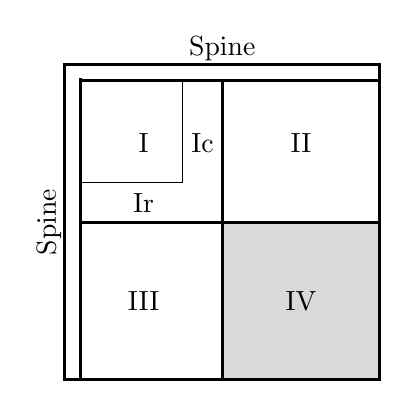
\begin{tikzpicture}
      \colorlet{fill}{gray!30}
      \colorlet{blank}{white}
      \fill[color=fill] (4,0) rectangle (4,-2);
      \fill[color=fill] (2,-2) rectangle (4,-4);
      \draw[very thick, step=2] (0, 0) grid (4, -4);
      \draw (0, -1.5) -- (1.5, -1.5);
      \draw (1.5, 0) -- (1.5, -1.5);
      \fill[color=white] (0,0) rectangle (0.2, -4);
      \fill[color=white] (0, 0) rectangle (4, -0.2);

      \draw[very thick, step=2] (0.2, -0.2) rectangle (0.2, -4);
      \draw[very thick, step=2] (0.2, 0) rectangle (4, -0.2);
      \fill[color=white] (0, 0) rectangle (4, -0.17);

      \draw[very thick, step=2] (0, 0) rectangle (4, -4);

      \node at (1,-1)    {I};
      \node at (1,-1.75) {Ir};
      \node at (1.75,-1) {Ic};
      \node at (1,-3)    {III};
      \node at (3,-3)    {IV};
      \node at (3,-1)    {II};
      \node[rotate=90] at (-0.2, -2)  {Spine};
      \node at (2, 0.2)  {Spine};
    \end{tikzpicture}
    \caption{Regions of the board}\label{fig:regions}
  \end{subfigure}
  \begin{subfigure}[b]{0.4\textwidth}
    \centering
    %\input{papers/calibration.pdf_t}
    \caption{An example of normal play}\label{fig:normal-play}
  \end{subfigure}
  \caption{Regions to constrain the players.  Each `block' is a $n \times n$ square.% with $n = 2k + 1$.%Taken as a variant of \lang{RCG'},
  }
\end{figure}

\subsection{Normal Play}

By a \emph{round}, we mean a pair of consecutive turns, starting with Rose.  We index the rounds starting with round~$0$.  Normal play is in three stages:
\begin{description}
  \item[Spine:]
        In round~$0$, both players play the spine, i.e., a string matching $\2\1\0^*$.
  \item[Calibration:]
        In round~$i$, where $1\le i\le n$, Rose and Colin each play a `calibration string,' i.e. either the string matching $\0^i\1^3\0^{n-i-2}\|\0^i\1\0^{n-i-1}$ (if $i<n$) or $\0\0^{n-2}\1\1\|\0^{n-1}\1$ (if $i=n$).
  \item[Simulation:] Rose and Colin now simulate the given
        $\lang{\RCG'}$ game: In round~$(n+i)$, for $1\le i\le n$, Rose plays
        a string matching $\0^i\1\0^{n-i-1}\|R_i$ (if she can), and Colin plays a string matching $\0^i\1\0^{n-i-1}\|C_i$ (if he can).
\end{description}

Figure~\ref{fig:normal-play} illustrates the state of the grid after round~$n$ of normal play (here, $n=16$). If either player deviates from normal play, we say that the first player to do so is \emph{cheating}.  The next lemmas show that Colin cannot cheat, and if Rose cheats, then Colin can force her to lose in a constant number of rounds by playing a \emph{bomb}, i.e., a string matching $(\0 \cup \1 \cup \1\0\0\cup \0\0^*\1\0)\2^*$, once or twice.

\begin{lemma}\label{lem:spine}
  In round~$0$, if Rose does not play the spine, then Colin can win; otherwise, Colin must also play the spine.
\end{lemma}
\begin{proof}
  If Rose does not play $\2\1\0^*$, she has two choices for the first character. If she chooses $0$, say, then Colin has a quick kill by playing a bomb (see Figure~\ref{fig:bomb}), with similar results if she cheats with a $1$.
  \begin{figure}[H]
    \centering
    0:
    \begin{subfigure}[c]{0.25\textwidth}
      \centering
      \DrawGame{(0,0)}{(4,-1)}{
        {     0, ?, ?, ?},
        {      , , , },
        {      , , , },
        {      , , , },
      }
      \vspace{2.5mm}
    \end{subfigure}
    \begin{subfigure}[c]{0.25\textwidth}
      \centering
      \DrawGame{(0,0)}{(1,-4)}{
        {     0, ?, ?, ?},
        {     2, , , },
        {     2, , , },
        {     2, , , },
      }
      \vspace{2.5mm}
    \end{subfigure}
    \\
    1:
    \begin{subfigure}[c]{0.25\textwidth}
      \centering
      \DrawGame{(0,-1)}{(4,-2)}{
        {     0, ?, ?, ?},
        {     2, 1, 0, 0},
        {     2, , , },
        {     2, , , },
      }
      \vspace{2.5mm}
    \end{subfigure}
    \begin{subfigure}[c]{0.25\textwidth}
      \centering
      \DrawGame{(1,-0)}{(2,-4)}{
        {     0, 1, ?, ?},
        {     2, 1, 0, 0},
        {     2, 1, , },
        {     2, 0, , },
      }
      \vspace{2.5mm}
    \end{subfigure}
    \\
    2:
    \begin{subfigure}[c]{0.25\textwidth}
      \centering
      \DrawGame{(0,-2)}{(4,-3)}{
        {     0, 1, ?, ?},
        {     2, 1, 0, 0},
        {     2, 1, 0, 0 },
        {     2, 0, , },
      }
    \end{subfigure}
    \begin{subfigure}[c]{0.25\textwidth}
      \centering
      \DrawGame{(2,0)}{(3,-4)}{
        {     0, 1, 1, ?},
        {     2, 1, 0, 0},
        {     2, 1, 0, 0 },
        {     2, 0, 2, },
      }
    \end{subfigure}
    \caption{Each round when Rose cheats with $0\cdots$ in her first move and Colin plays a bomb. Note that Rose has no regex to match the prefix $20$. We replace a `?' with a $1$ in round~$1$ to show the worst case, where Colin must survive through round~$2$ (not required in the $0$ case).}\label{fig:bomb}
  \end{figure}
  In either case, Rose would quickly lose. If Rose does play $\2\1\0^*$ on her first turn, Colin must play a string prefixed with $2$, his only option matching the regex $\2\1\0^*$.
\end{proof}
\begin{lemma}\label{lem:bomb}
  After normal play through round~$(i-1)$ for $1\le i\le n$, Rose prefers regex~(\ref{eqn:ros-cal1}) to regex~(\ref{eqn:ros-generic}) in round~$i$.
\end{lemma}
\begin{proof}
  If $i=1$, then Rose must play a string with prefix $1$, and so she must play a string matching regex~(\ref{eqn:ros-cal1}).  Now suppose $i\ge 2$, and consider the following portion of the board at the start of round~$i$ when both players have been playing normally:
  \begin{figure}[H]
    \centering
    \DrawMidGame{(0,0)}{(0,0)}{
      {1,1,0,0},
      {1,1,1,0},
      {0,1, , },
      {0,0, , },
    }
  \end{figure}
  Rose has a choice of regexes~(\ref{eqn:ros-cal1}) or~(\ref{eqn:ros-generic}), as each can match a string prefixed by $0^{i-1}1$. Say Rose chooses regex~(\ref{eqn:ros-generic}), thus playing a string matching $\0^{i-1}\1\0^{n-i} \| R_{i-1}$.  Colin can then respond with a bomb:
  \begin{figure}[H]
    \centering
    \begin{subfigure}[t]{0.25\textwidth}
      \centering
      \DrawMidGame{(0,-2)}{(4,-3)}{
        {1,1,0,0},
        {1,1,1,0},
        {0,1,0,0},
        {0,0, , },
      }
      \caption{Rose plays regex~(\ref{eqn:ros-generic})}
    \end{subfigure}
    \hspace{2cm}
    \begin{subfigure}[t]{0.25\textwidth}
      \centering
      \DrawMidGame{(2,0)}{(3,-4)}{
        {1,1,0,0},
        {1,1,1,0},
        {0,1,0,0},
        {0,0,2, },
      }
      \caption{Colin plays regex~(\ref{eqn:col-bomb}), Rose loses}
    \end{subfigure}
  \end{figure}
  Rose cannot then play any string with prefix $0^i2$, so she loses in round~$(i+1)$.
\end{proof}
\begin{lemma}
  Colin cannot cheat in rounds $1$ through $n$.
\end{lemma}
\begin{proof}
  By Lemma~\ref{lem:spine}, we begin round 1 with the spine having been played by both players. Rose is then forced to play a string prefixed with $1$, the only matching regex being regex~(\ref{eqn:ros-cal1}) with $i = 0$: $\1\1\1\0^{n-2} \| \1\0^{n-1}$.  From this point on through round~$n$, assuming Rose plays normally, Colin will be faced with prefix $0^{i-1}11$ in round~$i$, and thus must play a string matching regex~(\ref{eqn:col-cal1}) or (\ref{eqn:col-cal2}), i.e., play normally.
\end{proof}

The preceding lemmas show that normal play is optimal for both players (even required for Colin) through round~$n$.  Thus we can assume normal play through round~$n$, filling regions II and III of the grid with $1$'s along their diagonals and $0$'s elsewhere (as with the identity matrix).

\begin{lemma}
  Assume normal play through round~$n$.  For $1\le i\le n$, in round~$(n+i)$, Rose must play a string matching $\0^i\1\0^{n-i}\|R_i$ and Colin must play a string matching $\0^i\1\0^{n-i}\|C_i$.
\end{lemma}
\begin{proof}
  In round~$(n+i)$, Rose and Colin are both faced with prefix $0^i10^{n-i}$, and the only regexes that this matches are the respective regexes given above for Rose and Colin.
\end{proof}

In rounds~$(n+1)$ through $2n$, the players are essentially playing the game $G$ in region IV, so the winner of $H$ is the winner of $G$. This completes the proof of Theorem~\ref{thm:constant-regexes}.

\section{Open Problems}\label{sec:open}

The most immediate question arising from our work is whether \lang{RCG} is \lang{PSPACE}-hard restricted to a binary alphabet.  Our proof shows only that it is \lang{PSPACE}-hard for a ternary alphabet. Doing without the third symbol ``$2$'' in the alphabet currently seems like a daunting task, despite the fact that under normal play, that symbol appears only once in the upper left-hand corner.

Another question is whether we still get \lang{PSPACE}-hardness if we restict the regexes $R$ and $C$ to be equal to each other.  If one can show \lang{PSPACE}-hardness for \lang{RCG'} restricted so that $R_i = C_i$ for all $i$, then it may be easy to get $R=C$ for the constructed instance of \lang{RCG}, since these two latter regexes are close to being equal anyway.

\section*{Acknowledgments}

We would like to thank Thomas Thierauf for several interesting discussions on this topic and to Joshua Cooper for finding for us a particularly challenging and fun regex crossword puzzle.  We are also grateful to Klaus-J\"orn Lange for suggesting the connection between our work and the theory of picture languages.

\nocite{*}
\bibliographystyle{alpha}
\bibliography{papers/rc-cross}
\end{document}
